% !TeX program = pdflatex
% Compilar dos veces con pdflatex desde esta carpeta.
% Primera propuesta basada en la memoria anual, versión del 24/11/2026.
\documentclass[aspectratio=169,11pt]{beamer}
\usepackage[utf8]{inputenc}
\usepackage[T1]{fontenc}
\usepackage[spanish]{babel}
\usepackage{lmodern,graphicx,booktabs,amsmath,array}
\usepackage{tikz}
\graphicspath{{figs/}}
\definecolor{navy}{HTML}{16364B}
\definecolor{teal}{HTML}{007F86}
\definecolor{muted}{HTML}{52616B}
\setbeamercolor{normal text}{fg=navy,bg=white}
\setbeamercolor{structure}{fg=teal}
\setbeamercolor{frametitle}{fg=navy}
\setbeamercolor{title}{fg=navy}
\setbeamercolor{alerted text}{fg=teal}
\setbeamerfont{frametitle}{size=\Large,series=\bfseries}
\setbeamerfont{title}{size=\LARGE,series=\bfseries}
\setbeamertemplate{navigation symbols}{}
\setbeamertemplate{itemize item}{\small\textbullet}
\setbeamertemplate{itemize subitem}{\small\textbullet}
\setbeamersize{text margin left=9mm,text margin right=9mm}
\setbeamertemplate{frametitle}{\vspace{4mm}\insertframetitle\par\vspace{1mm}}
\setbeamertemplate{footline}{\hspace{9mm}\scriptsize\color{muted}TIMPRE\quad Memoria 2026\hfill\insertframenumber\,/\,\inserttotalframenumber\hspace{9mm}\vspace{3mm}}
\setlength{\parskip}{5pt}
\newcommand{\source}[1]{{\par\vspace{1mm}\fontsize{7}{8}\selectfont\color{muted}#1\par}}
\newcommand{\takeaway}[1]{{\par\vspace{2mm}\color{teal}\bfseries #1\par}}
\newcommand{\fig}[2][5.1cm]{{\centering\includegraphics[width=\linewidth,height=#1,keepaspectratio]{#2}\par}}
\title{Memoria anual 2026}
\subtitle{Tecnología de imagen multimodal\\para investigación preclínica}
\author{Guillermo G. Cosarinsky Markman}
\institute{TIMPRE · Programa Momentum CSIC}
\date{2026}
\begin{document}

% 01 -----------------------------------------------------------------
\begin{frame}[plain]
\par\vspace{5mm}
{\color{teal}\large TIMPRE\quad /\quad Momentum CSIC\par}
\par\vspace{6mm}
{\usebeamerfont{title}\inserttitle\par}
\par\vspace{3mm}
{\large Formación de imagen ultrasónica con IA\\y guiado ecocardiográfico\par}
\par\vspace{5mm}
\insertauthor\par
\vfill

\includegraphics[width=.86\textwidth]{logos_todos.png}
\par\vspace{3mm}
\note{Presentar el trabajo de 2026 como continuidad del estudio de NSI y apertura de la línea de asistencia a la adquisición. El contenido sigue la memoria anual disponible el 24 de noviembre.}
\end{frame}

% 02 -----------------------------------------------------------------
\begin{frame}{Contribución al proyecto TIMPRE}
\relax
{\large El trabajo de 2026 se centra en el\newline\alert{componente ultrasónico de la imagen multimodal}.\par}
\par\vspace{3mm}
\centering
\begin{tikzpicture}[x=1cm,y=1cm,
 branch/.style={align=left,text width=5.5cm,font=\fontsize{10}{12}\selectfont,inner sep=0pt},
 link/.style={thick,draw=teal},
 flow/.style={->,>=stealth,thick,draw=teal}]
\node[branch,anchor=north] (formation) at (3,0) {\textbf{Formación de imagen}\\\textbf{(beamforming)}};
\node[branch,anchor=north] (guidance) at (10,0) {\textbf{Asistencia a la adquisición}\\\textbf{en ecocardiografía}};
\node[align=center,text width=9cm,draw=teal,fill=teal!5,rounded corners=2pt,inner sep=7pt,font=\fontsize{11}{13}\selectfont] (common) at (6.5,-1.90) {\textbf{Base metodológica común}\\Herramientas de simulación y aprendizaje automático};
\draw[link] (formation.south)--(3,-1.00)--(6.5,-1.00);
\draw[link] (guidance.south)--(10,-1.00)--(6.5,-1.00);
\draw[flow] (6.5,-1.00)--(common.north);
\node[align=center,text width=10cm,font=\fontsize{11}{13}\selectfont] (preclinical) at (6.5,-3.37) {\textbf{Posibles aplicaciones futuras en imagen preclínica}\\Mejora de la formación de imagen y asistencia a la adquisición};
\draw[flow,dashed] (common.south)--(preclinical.north);
\end{tikzpicture}
\note{Ambas líneas comparten herramientas de simulación y aprendizaje automático. Esta base metodológica puede contribuir también a futuras aplicaciones preclínicas de formación de imagen y asistencia a la adquisición. La conexión con la multimodalidad es metodológica: el trabajo no ha realizado una integración entre modalidades ni una validación preclínica del guiado. La flecha discontinua señala esa proyección futura.}
\end{frame}

% 03 -----------------------------------------------------------------
\begin{frame}{Actividades de 2026}
\relax
\begin{tabular}{@{}>{\raggedright\arraybackslash}p{.24\textwidth}>{\raggedright\arraybackslash}p{.67\textwidth}@{}}
\textbf{TFM} & Diseño de una apodización de recepción mediante una representación neuronal implícita (INR).\\[5mm]
\textbf{Tecniacústica} & Extensión a múltiples apodizaciones y una combinación neuronal de imágenes.\\[5mm]
\textbf{Estancia UCM} & Revisión de métodos de guiado, simulación de ecocardiografía y segmentación anatómica.\\[5mm]
\textbf{Formación y difusión} & Finalización del máster en IA Aplicada y participación en SABIA 2026.
\end{tabular}\par
\end{frame}

\section{Formación de imagen con IA}
% 04 -----------------------------------------------------------------
\begin{frame}{NSI: tres apodizaciones de recepción}
\relax
\fig[3.6cm]{nsi_apodizaciones_lineales.pdf}
\par\vspace{1mm}
\begin{itemize}
\item La apodización asigna un peso a la señal de cada elemento antes de sumarla.
\item La distribución de media cero genera un nulo central bajo condiciones de simetría.
\end{itemize}
\source{Agarwal et al., IEEE TUFFC, 2019. Ejemplo de la memoria: 64 elementos y $dc=0{,}1$.}
\end{frame}

% 05 -----------------------------------------------------------------
\begin{frame}{NSI: combinación de las envolventes}
\relax
\par\vspace{-2mm}
\[I_{\mathrm{NSI}}=\tfrac12\bigl(|I_{dc1}|+|I_{dc2}|\bigr)-|I_{zm}|\]
\fig[3.8cm]{nsi_perfil_final_uniforme.pdf}
\source{Modelo ideal de campo lejano: $N=64$, $dc=0{,}1$, $d=2\lambda$. Cada perfil final se normaliza por su máximo, después de la combinación. Ventana angular alrededor del enfoque.}
\note{Explicar que el estrechamiento corresponde a este modelo simétrico. Las amplitudes se combinan antes de normalizar y la figura no representa una evaluación funcional.}
\end{frame}

% 06 -----------------------------------------------------------------
\begin{frame}{Limitación cerca de los extremos del array}
\relax
\setlength{\parskip}{2pt}
\fig[3.7cm]{nsi_apodization_profiles.png}
{\small\textbf{(a)} Recorte simétrico cerca del borde.\quad
\textbf{(b)} Sin recorte, lejos del borde.\par}
\begin{itemize}
\item El recorte simétrico conserva el equilibrio entre pesos positivos y negativos, pero reduce la apertura efectiva.
\end{itemize}
\takeaway{Motivación: aprender apodizaciones adaptadas a la geometría disponible.}
\source{Figura del artículo de Tecniacústica 2026. Líneas rojas: límites del array; línea gris: centro de la subapertura.}
\note{La figura muestra la apodización de media cero de NSI en dos posiciones laterales. En (a), x=-17,1 mm, la restricción de simetría reduce la apertura para mantener el equilibrio entre los pesos. En (b), x=-6,1 mm, la subapertura no está recortada. Distinguir esta reducción simétrica de un recorte unilateral que desequilibraría los pesos y alteraría la cancelación.}
\end{frame}

% 07 -----------------------------------------------------------------
\begin{frame}{TFM: una apodización representada por una INR}
\relax
\begin{columns}[c,onlytextwidth]
\column{.51\textwidth}
\fig[5.3cm]{tfm_esquema_inr.png}
\column{.45\textwidth}
Una red calcula el peso a partir de la posición del píxel y del elemento receptor.
\[a_{\mathrm{INR}}(x,z,x_{elem})\]
\begin{itemize}
\item MLP de tres capas ocultas de 8 neuronas.
\item Pesos reales entre 0 y 1.
\item Integración en retardo y suma (DAS).
\end{itemize}
\end{columns}
\source{TFM, Cosarinsky, 2026. Entradas geométricas: $|x|$, $z$ y $|x-x_{elem}|$.}
\end{frame}

% 08 -----------------------------------------------------------------
\begin{frame}{TFM: aprendizaje con reflectores simulados}
\relax
\begin{columns}[T,onlytextwidth]
\column{.47\textwidth}
\textbf{Datos de entrenamiento}
\begin{itemize}
\item Sonda lineal de 128 elementos.
\item 100 escenarios con 100 reflectores cada uno.
\item 11 ondas planas entre $-5^\circ$ y $5^\circ$.
\item 20\% de escenarios para validación.
\end{itemize}
\column{.47\textwidth}
\textbf{Objetivo de aprendizaje}
\par Imagen DAS uniforme multiplicada por máscaras gaussianas centradas en los reflectores.
\par Error absoluto ponderado y regularización para evitar la supresión indiscriminada de señal.
\end{columns}
\par\vspace{4mm}
\takeaway{Prueba de concepto en un medio homogéneo con posiciones conocidas.}
\source{TFM, Cosarinsky, 2026. Simulación con PyMUST; optimización Adam, 40 épocas.}
\end{frame}

% 09 -----------------------------------------------------------------
\begin{frame}{TFM: comparación de las imágenes DAS}
\relax
\begin{columns}[c,onlytextwidth]
\column{.65\textwidth}
\fig[5.6cm]{tfm_comparacion_imagenes.png}
\column{.31\textwidth}
\textbf{Misma grilla simulada}
\par Uniforme\par Hanning dinámica\par Rectangular dinámica\par INR
\par\vspace{3mm}
La distribución aprendida combina una apertura variable con la profundidad y una ponderación suave.
\end{columns}
\source{Figura del TFM, 2026. Escala de amplitud en dB indicada en la figura.}
\end{frame}

% 10 -----------------------------------------------------------------
\begin{frame}{TFM: resolución lateral y SNR}
\relax
\fig[3.8cm]{tfm_comparacion_metricas.png}
\begin{itemize}
\item Frente a Hanning: respuestas más estrechas, con SNR próxima y algo inferior en profundidad.
\item Frente a uniforme: mayor SNR, acompañada de respuestas generalmente más anchas.
\end{itemize}
\source{TFM, 2026. FWHM y SNR según las definiciones del trabajo, evaluadas por reflector en la grilla simulada.}
\end{frame}

% 11 -----------------------------------------------------------------
\begin{frame}{Tecniacústica: múltiples apodizaciones y mixer}
\relax
\fig[3.35cm]{tecni_arquitectura.png}
\[I_m=\sum_j a_m(x,z,x_{elem}(j))\,s_{ret}(x,z,j),\qquad
I_{final}=g_\phi\bigl(|I_1|,\ldots,|I_M|\bigr)\]
\takeaway{Se aprenden los pesos de recepción y la combinación de las envolventes.}
\source{Artículo de Tecniacústica 2026. El esquema ilustra tres apodizaciones; la configuración evaluada utiliza dos.}
\end{frame}

% 12 -----------------------------------------------------------------
\begin{frame}{Tecniacústica: entrenamiento y evaluación}
\relax
\begin{columns}[T,onlytextwidth]
\column{.47\textwidth}
\textbf{Entrenamiento}
\begin{itemize}
\item Reflectores puntuales simulados con PyMUST.
\item Geometría de la sonda PICMUS y 11 ondas planas.
\item Referencia DAS con máscara gaussiana.
\item Ventana Hanning dinámica, $F_{\#}=1$, aplicada a los pesos aprendidos.
\end{itemize}
\column{.47\textwidth}
\textbf{Evaluación}
\begin{itemize}
\item Grilla de reflectores simulados.
\item Adquisición experimental de un fantoma PICMUS.
\item Comparación con DAS Hanning y NSI.
\item Atención a los reflectores próximos al borde lateral.
\end{itemize}
\end{columns}
\source{Artículo de Tecniacústica 2026. INR: capas ocultas de 16, 8 y 4 neuronas; dos apodizaciones y mixer de dos capas ocultas.}
\end{frame}

% 13 -----------------------------------------------------------------
\begin{frame}{Mejoras locales cerca del borde en simulación}
\relax
\fig[3.9cm]{tecni_resultados_borde.png}
\begin{itemize}
\item Respuesta más estrecha que NSI en el reflector mostrado, $x=18$ mm y $z=30$ mm.
\item La caída de amplitud de NSI con la profundidad no aparece en el método aprendido.
\end{itemize}
\source{Tecniacústica 2026. Extremo del array: $x=19{,}5$ mm. Amplitudes relativas al primer reflector de la columna.}
\note{La ventaja es local. NSI conserva el mejor comportamiento en la mayor parte de la imagen simulada. No generalizar este resultado a toda la grilla.}
\end{frame}

% 14 -----------------------------------------------------------------
\begin{frame}{Evaluación experimental en PICMUS}
\relax
\begin{columns}[c,onlytextwidth]
\column{.67\textwidth}
\fig[5.5cm]{tecni_resultados_picmus.png}
\column{.29\textwidth}
\textbf{Resultado global}
\par NSI ofrece la mejor resolución lateral.
\par El método aprendido resulta, en conjunto, comparable a DAS.
\par\vspace{2mm}
\textbf{Cerca del borde}
\par Mejoras locales menores que en simulación.
\end{columns}
\source{Artículo de Tecniacústica 2026. Fantoma PICMUS; perfiles de reflectores seleccionados en $x=20$ mm.}
\end{frame}

% 15 -----------------------------------------------------------------
\begin{frame}{Balance del trabajo en beamforming}
\relax
\begin{tabular}{@{}>{\raggedright\arraybackslash}p{.24\textwidth}>{\raggedright\arraybackslash}p{.68\textwidth}@{}}
\textbf{TFM} & Una INR aprende una apodización dependiente de la geometría y un compromiso entre anchura lateral y SNR.\\[5mm]
\textbf{Tecniacústica} & El aprendizaje conjunto de apodizaciones y combinación muestra ventajas locales cerca del borde.\\[5mm]
\textbf{Alcance} & El TFM se limita a simulación. La extensión experimental sigue siendo preliminar y no supera globalmente a NSI.
\end{tabular}\par
\par\vspace{4mm}
\takeaway{Base para estudiar otras arquitecturas y objetivos de entrenamiento.}
\end{frame}

\section{Guiado ecocardiográfico}
% 16 -----------------------------------------------------------------
\begin{frame}{Estancia de investigación en la UCM}
\relax
{\large Grupo del profesor Joaquín López Herraiz\par}
Departamento de Estructura de la Materia, Física Térmica y Electrónica.
\par\vspace{3mm}
\par\textbf{Periodo previsto:} 16 de septiembre a 11 de diciembre de 2026.
\par\vspace{5mm}
\begin{itemize}
\item Investigar métodos de IA para asistir al operador durante la adquisición ecocardiográfica.
\item Establecer un entorno de simulación y evaluación.
\item Estudiar criterios anatómicos para definir las vistas objetivo.
\end{itemize}
\note{La estancia está en curso en la fecha de preparación. No presentar el periodo completo como ya realizado.}
\end{frame}

% Vista anatómica: recorte del panel de la primera fila, segunda columna.
% Original: 1897 x 757 px, 72 dpi. Región: x=[481,940), y=[8,372).
\begin{frame}{Vista apical de cuatro cámaras (A4C)}
\relax
\begin{columns}[c,onlytextwidth]
\column{.53\textwidth}
\centering
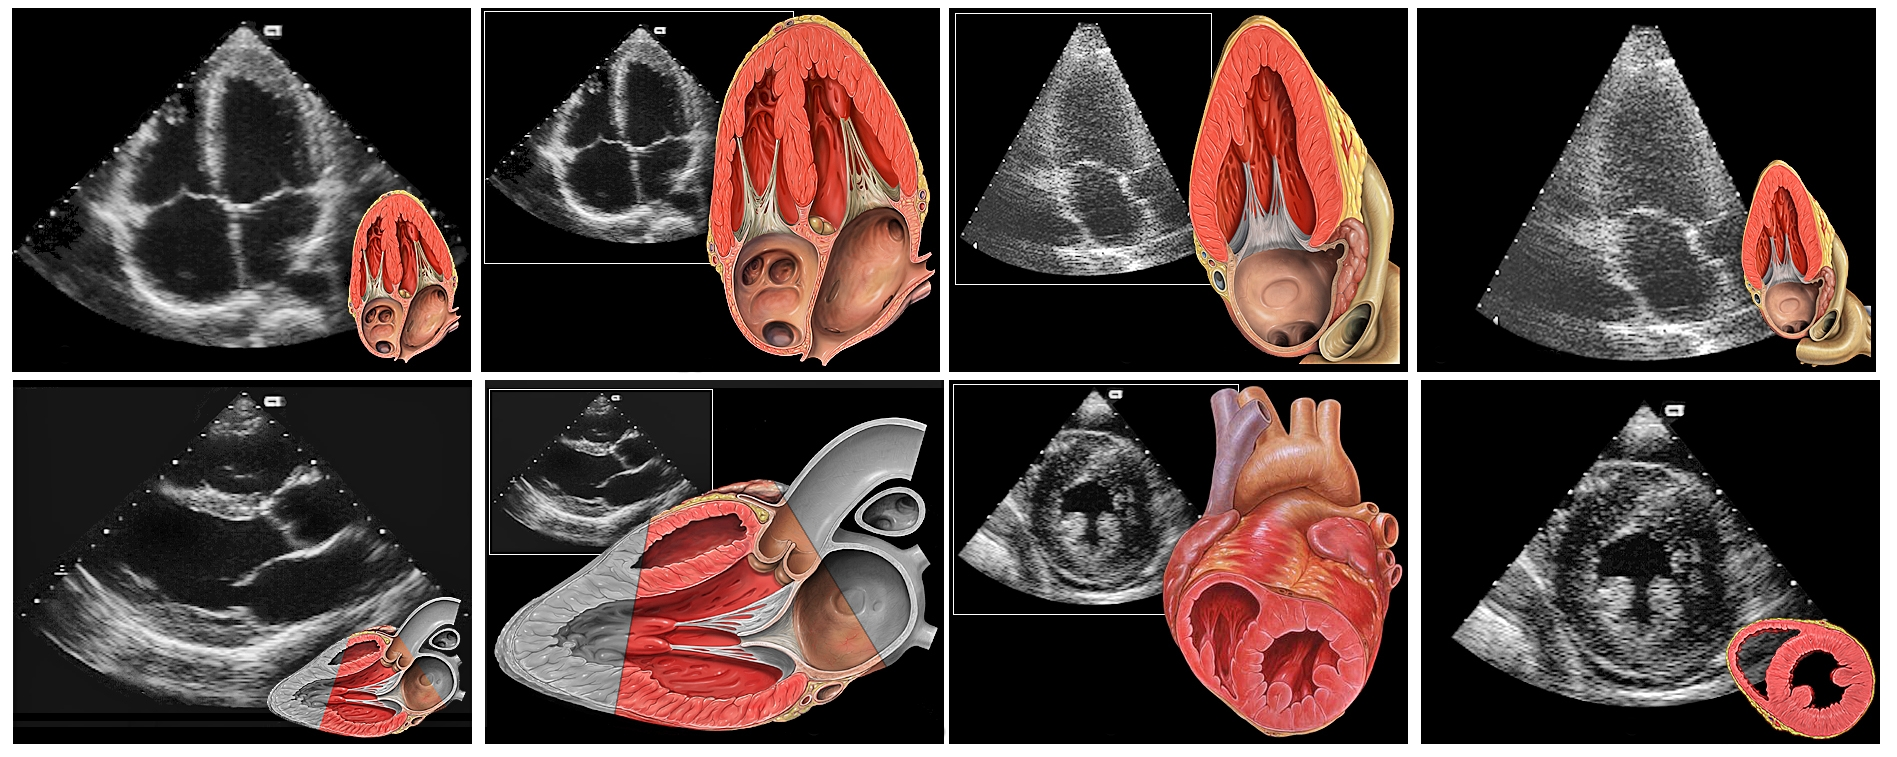
\includegraphics[width=\linewidth,height=4.9cm,keepaspectratio,trim={481bp 385bp 957bp 8bp},clip]{heart_normal_tte_views_original.jpg}
\column{.43\textwidth}
\textbf{Contenido anatómico}
\par Ventrículos izquierdo y derecho, aurículas izquierda y derecha, y válvulas mitral y tricúspide.
\par\vspace{3mm}
\textbf{Objetivo del guiado}
\par Ajustar la posición y la orientación de la sonda para obtener una vista anatómicamente adecuada.
\end{columns}
\source{Ilustración: Patrick J. Lynch y C. Carl Jaffe. \href{https://commons.wikimedia.org/wiki/File:Heart_normal_tte_views.jpg}{Wikimedia Commons}. \href{https://creativecommons.org/licenses/by/2.5/}{CC BY 2.5}. Recorte de la primera fila, segunda columna.}
\end{frame}

% 17 -----------------------------------------------------------------
\begin{frame}{Guiado: estimar una corrección de la sonda}
\relax
\begin{columns}[T,onlytextwidth]
\column{.48\textwidth}
\textbf{Observaciones}
\par Imagen actual o historial de imágenes ecográficas.
\par\vspace{3mm}
\textbf{Salida deseada}
\par Traslación y rotación, o maniobras discretas, para aproximarse a una vista válida.
\column{.46\textwidth}
\textbf{Referencia geométrica}
\[\Delta T_t=T_t^{-1}T_{\star,v}\]
\small $T_t$: pose actual.\par
$T_{\star,v}$: una pose válida para la vista $v$ en ese paciente.
\end{columns}
\par\vspace{5mm}
\takeaway{Una vista estándar se define por su anatomía; la pose que la produce varía entre pacientes.}
\source{Formulación y revisión bibliográfica de la memoria 2026.}
\note{El sistema visual planteado debe inferir la corrección desde las imágenes. Las poses del simulador pueden servir como etiquetas o para evaluar; esto no implica que estén disponibles durante el uso.}
\end{frame}

% 18 -----------------------------------------------------------------
\begin{frame}{Antecedentes: cómo se aprende el guiado}
\relax
\setlength{\parskip}{2pt}
{\small\textbf{Entrada del modelo, según el método:} imágenes o imágenes + pose.\par}
\vspace{2mm}
\centering
\begin{tikzpicture}[x=1cm,y=1cm,
 box/.style={draw=navy!40,rounded corners=2pt,align=center,minimum height=.65cm,font=\fontsize{9}{10}\selectfont,inner sep=5pt},
 flow/.style={->,>=stealth,thick,draw=teal},
 caption/.style={font=\fontsize{9}{10}\selectfont,text=navy,anchor=west}]
\node[anchor=west,text=teal,font=\bfseries] at (0,0) {Aprendizaje supervisado};
\node[box,text width=1.8cm] (sm) at (1.2,-.65) {Modelo};
\node[box,text width=2cm] (sp) at (4.5,-.65) {Maniobra predicha};
\node[box,text width=4.4cm,draw=teal] (sl) at (10,-.65) {Comparación con la\\\textbf{maniobra correcta etiquetada}};
\draw[flow] (sm)--(sp);
\draw[flow] (sp)--(sl);
\draw[flow] (sl.south)--(10,-1.3)--node[below,font=\fontsize{8}{9}\selectfont]{Ajustar el modelo para aprender las maniobras etiquetadas}(1.2,-1.3)--(sm.south);
\node[anchor=west,text=teal,font=\bfseries] at (0,-2.05) {Aprendizaje por refuerzo};
\node[box,text width=1.8cm] (rm) at (1.2,-2.85) {Modelo};
\node[box,text width=1.65cm] (ra) at (4.2,-2.85) {Movimiento};
\node[box,text width=2.7cm] (re) at (7.4,-2.85) {Entorno simulado\\\textbf{Nueva vista}};
\node[box,text width=2.5cm,draw=teal,fill=teal!5] (reward) at (11.15,-2.85) {\textbf{Recompensa}\\Acercamiento\\a la vista objetivo};
\draw[flow] (rm)--(ra);
\draw[flow] (ra)--(re);
\draw[flow] (re)--(reward);
\draw[flow] (re.south)--(7.4,-3.5)--node[below,font=\fontsize{8}{9}\selectfont]{Nueva observación}(1.2,-3.5)--(rm.south);
\node[caption] at (0,-4.12) {Aprender secuencias que maximicen la \textbf{recompensa acumulada}.};
\end{tikzpicture}
\par\vspace{1mm}
\raggedright
{\fontsize{10}{12}\selectfont\color{teal}\bfseries Nuestro objetivo: solo imágenes, sin medición externa de la pose.\par}
\vspace{1mm}
{\fontsize{8}{10}\selectfont En entrenamiento, las poses del simulador pueden generar etiquetas, calcular recompensas o evaluar movimientos, sin ser entradas del modelo.\par}
\note{Esquemas de entrenamiento. La entrada, común a ambos esquemas y dependiente del método, puede ser imágenes o imágenes y pose. En supervisado se aprende a reproducir maniobras etiquetadas. En refuerzo, tras cada movimiento, el simulador produce una nueva vista y se obtiene una recompensa que valora el acercamiento al objetivo. El modelo aprende secuencias que maximicen la recompensa acumulada. Nuestro objetivo de uso es únicamente visual, sin instrumentación externa de seguimiento. Las poses conocidas del simulador pueden utilizarse durante el entrenamiento sin constituir entradas del modelo. Referencias: sección 3.2 de la memoria anual 2026.}
\end{frame}

% 19 -----------------------------------------------------------------
\begin{frame}{Criterios anatómicos para definir la meta}
\relax
\textbf{Propuesta revisada de Cao et al.}
\par Proporciones de áreas y relaciones espaciales extraídas de segmentaciones de vistas estándar.
\par Sus distribuciones estadísticas definen el estado y la recompensa de una política.
\par\vspace{2mm}
\textbf{Interés para el proyecto}
\par Definir con los médicos las características de una vista aceptable y la precisión necesaria.
\takeaway{Primer paso: segmentación de cavidades y válvulas en simulación.}
\source{Cao et al., 2026, según la revisión de la memoria. Demostración del antecedente limitada a rotaciones de A4C en simulación y fantoma.}
\end{frame}

% 20 -----------------------------------------------------------------
\begin{frame}{TARTAGLIA 2D: entorno de experimentación}
\relax
\fig[3.7cm]{panel_simulador_tartaglia.png}
\begin{itemize}
\item Control de posición, orientación de la sonda y fase cardíaca.
\item Imágenes B-mode, etiquetas anatómicas y poses conocidas.
\item Dos casos virtuales disponibles; nuevos casos en preparación.
\end{itemize}
\source{Simulador del grupo UCM. Renderizado mediante respuestas PSF precalculadas; no genera señales por canal. Referencias geométricas pendientes de revisión anatómica.}
\note{La anatomía torácica procede de CT y el corazón se incorpora a partir de CONRAD. No describirlo como una segmentación directa del corazón de ese CT. La imagen ilustrada es una referencia geométrica, no una certificación clínica de la vista.}
\end{frame}

% 21 -----------------------------------------------------------------
\begin{frame}{Segmentación de la vista A4CH}
\relax
\begin{columns}[T,onlytextwidth]
\column{.47\textwidth}
\textbf{Modelo}
\begin{itemize}
\item U-Net de CASTOR preentrenada en CAMUS.
\item Salida adaptada a siete clases: fondo, cuatro cavidades y dos válvulas.
\item Entrada B-mode de $512\times512$ píxeles.
\item Sin poses ni información temporal.
\end{itemize}
\column{.47\textwidth}
\textbf{Datos y entrenamiento}
\begin{itemize}
\item Caso A: 1.280 imágenes de 256 poses.
\item 896 de entrenamiento, 192 de validación y 192 de prueba.
\item Poses separadas entre particiones; fases de cada pose juntas.
\item Entropía cruzada ponderada y pérdida Dice.
\end{itemize}
\end{columns}
\source{Experimento CASTOR descrito en la memoria 2026. Evaluación adicional en 192 imágenes de una segunda anatomía, B.}
\end{frame}

% 22 -----------------------------------------------------------------
\begin{frame}{Segmentación: poses de prueba del caso A}
\relax
\fig[5.35cm]{castor_segmentacion_caso_A.pdf}
\source{Dos poses de prueba del caso A. De izquierda a derecha: imagen B-mode, etiquetas del simulador y predicción. Anatomía utilizada para el entrenamiento, con poses de prueba separadas.}
\end{frame}

% 23 -----------------------------------------------------------------
\begin{frame}{Segmentación: transferencia al caso B}
\relax
\fig[5.35cm]{castor_segmentacion_caso_B.pdf}
\source{Mismo modelo, aplicado a una segunda anatomía. Persisten discrepancias de contorno, regiones espurias y errores de localización valvular.}
\end{frame}

% 24 -----------------------------------------------------------------
\begin{frame}{La precisión disminuye en la segunda anatomía}
\relax
\begin{columns}[c,onlytextwidth]
\column{.50\textwidth}
\small\renewcommand{\arraystretch}{1.10}
\begin{tabular}{@{}lrr@{}}
\toprule
\textbf{Estructura} & \textbf{Caso A} & \textbf{Caso B}\\
\midrule
\multicolumn{3}{@{}l}{\textit{Dice de solapamiento}}\\
VI & 0,96 & 0,88\\
VD & 0,95 & 0,78\\
AI & 0,94 & 0,78\\
AD & 0,95 & 0,59\\
Mitral & 0,56 & 0,29\\
Tricúspide & 0,54 & 0,17\\
\midrule
\multicolumn{3}{@{}l}{\textit{Surface Dice a 1 mm}}\\
Mitral & 0,95 & 0,54\\
Tricúspide & 0,94 & 0,42\\
\bottomrule
\end{tabular}\par
\column{.44\textwidth}
\textbf{192 imágenes por caso}
\par Entrenamiento únicamente en A.
\par Mejor resultado en cavidades que en válvulas.
\par La tolerancia de 1 mm es exploratoria.
\par\vspace{2mm}
\takeaway{Dos anatomías simuladas: evaluación inicial, sin validación clínica ni de guiado.}
\end{columns}
\source{Tabla de la memoria 2026. Medias sobre imágenes con la estructura presente; las predicciones vacías cuentan como cero.}
\end{frame}

\section{Formación y continuidad}
% 25 -----------------------------------------------------------------
\begin{frame}{Formación y cómputo de ECTS}
\relax
\renewcommand{\arraystretch}{1.5}
\begin{tabular}{@{}>{\raggedright\arraybackslash}p{.69\textwidth}r@{}}
\toprule
\textbf{Actividad} & \textbf{ECTS}\\
\midrule
Máster en IA Aplicada, módulos 5 a 10, incluido el TFM & 36\\
Estancia en la UCM, periodo previsto completo & 18,5\\
Memoria anual & 40\\
\midrule
\textbf{Total consignado en la memoria} & \textbf{94,5}\\
\bottomrule
\end{tabular}\par
\par\vspace{4mm}
\small Estancia: 58 días laborables de 8 horas = 464 horas.\par
A 25 horas por ECTS: 18,56 ECTS; se consignan 18,5, redondeados a la baja.
\source{Cómputo de la memoria 2026. El periodo previsto de la estancia termina el 11 de diciembre.}
\end{frame}

% 26 -----------------------------------------------------------------
\begin{frame}{Trabajos y participación científica}
\relax
\textbf{Trabajo de Fin de Máster}
\par Diseño de una apodización mediante INR, integrado en el Máster de Formación Permanente en IA Aplicada de la Universidad Europea.
\par\vspace{3mm}
\textbf{Tecniacústica 2026}
\par Presentación del trabajo sobre múltiples apodizaciones aprendidas y su combinación neuronal.
\par\vspace{3mm}
\textbf{SABIA 2026}
\par Participación en la organización del simposio y como chairman de una sesión.
\source{Memoria anual 2026. La memoria completa del TFM y el artículo de Tecniacústica figuran en sus anexos.}
\end{frame}

% 27 -----------------------------------------------------------------
\begin{frame}{Balance y continuidad}
\relax
\textbf{Trabajo realizado}
\begin{itemize}
\item Diseño de apodizaciones mediante redes neuronales y evaluación de su comportamiento.
\item Inicio de una línea de guiado ecocardiográfico apoyada en simulación y segmentación.
\end{itemize}
\par\vspace{5mm}
\textbf{Continuidad con la UCM}
\begin{itemize}
\item Ampliar el entrenamiento y la evaluación a nuevos casos simulados, reservando anatomías independientes.
\item Definir con los médicos criterios anatómicos y la precisión necesaria para incorporarlos al guiado.
\end{itemize}
\end{frame}
\end{document}
